%! suppress = MissingLabel

% Preamble
\documentclass[a4paper]{article}

\usepackage{geometry}
\geometry{
    a4paper,
    scale=0.8,
    bottom=2cm,
    top=2cm,
}

% Packages
\usepackage{amsmath}
\usepackage{csquotes}
\usepackage{natbib}
\usepackage{blindtext}
\usepackage{ctex}

\usepackage[utf8]{inputenc}
\usepackage[english]{babel}
\usepackage{indentfirst}
\usepackage{enumitem}
\usepackage{floatrow}
\usepackage{graphicx}
\usepackage{amsfonts}
\usepackage{amssymb}
\usepackage{listings}

% set up BNF generator
\usepackage{syntax}
\setlength{\grammarparsep}{10pt plus 1pt minus 1pt}
\setlength{\grammarindent}{10em}


\setlist{noitemsep} % removes spacing from items but leaves space around the whole list
%\setlist{nosep} % removes all vertical spacing within and around the list
\setlist[itemize]{topsep=0.25em, leftmargin=1.5pc}
\setlist[enumerate]{topsep=0.25em, leftmargin=1.5pc}

\renewcommand{\baselinestretch}{1.2}

%\setlength{\parindent}{0em}
\graphicspath{ {./} }

%! suppress = EscapeUnderscore
\newcommand*{\tproject}[1]{
    \begin{math}
        \pi_{#1}
    \end{math}
}

%! suppress = EscapeUnderscore
\newcommand*{\tselect}[1]{
    \begin{math}
        \sigma_{#1}
    \end{math}
}

\newcommand{\emptyline}{\\ \hspace*{\fill} \\}

\newcommand*{\textbfit}[1]{\textbf{\textit{#1}}}

\newcommand*{\seqdef}[1][a]{$({#1}_n)_{n\geq1}$}
\newcommand*{\subseqdef}[1][a]{$({{#1}_n}_i)_{i\geq1}$}
\newcommand*{\seq}[1][a]{#1_n}
\newcommand*{\limtoinf}[1][n]{\lim_{#1\rightarrow\infty}}
\newcommand{\abs}[1]{\left| #1 \right|}

\newcommand{\shell}[1]{\lstinline!#1!}
\usepackage{sourcecodepro}
\usepackage[T1]{fontenc}

\usepackage{hyperref}
\usepackage{xcolor}
\usepackage{textcomp}
\usepackage{caption}
\hypersetup{
    colorlinks,
    linkcolor={blue!50!black},
    citecolor={blue!50!black},
    urlcolor={blue!80!black}
}

\lstset{breaklines=true,basicstyle=\ttfamily\small,autogobble=true,language=C}

% Document
%! suppress = TooLargeSection
%! suppress = Quote
\begin{document}
    \title{
        \vspace{-3em}
        Human Centred Design Techniques Portfolio}
    \author{
        Group 43
    }
    \date{\vspace{-2em}}
    \maketitle

    \section*{The Problem}

    \noindent Jay, a computing student at Imperial College, is currently studying for his exams.
    He encountered a problem and attempted to get assistance from his friends, but they could not reach an agreement.
    Subsequently, he turned to Edstem, the school’s forum, to post a thread.
    Despite his expectation for a response from the tutors, he was left unanswered.
    He headed to the secret revision folder for help, but the solutions and comments there are unreadable due to their disorder.
    Alice, on the other hand, is a finance student from the LSE. She enjoys expressing her thoughts, but her lack of confidence inhibits her from posting responses publicly on the school forum.
    Moreover, she holds the belief that the tutors' responses are generally more authoritative.
    Thus, even when she could potentially provide useful insights to some questions, she often holds back, allowing the tutors to take the lead.\\
    \textbf{College students} are seeking a simplified method for verifying their solutions and an inclusive and comfortable environment where they can freely express their thoughts and contribute their ideas.

    From a tutor's perspective, the lack of responses is not by choice but a matter of necessity.
    Philip, a Graduate Teaching Assistant at UCL, explained,
    \begin{itemize}
        \item[-] ``I simply don't have enough time to respond to all posts, let alone provide immediate replies.''
        \item[-] ``I would prefer if some problems can be sorted by students discussing with each other.''
    \end{itemize}
    \textbf{Tutors} want to find a method that reduces the time required to respond all the posts, and peer conversations are encouraged.

    \textbf{The existing school forum presents challenges: it neither provides sufficient feedback for students nor encourages them to share ideas.
    Furthermore, it places undue pressure on the tutors.}

    \vspace*{1em}

    \noindent From the interviews conducted with college students, most candidates responded with the following:
    \begin{itemize}
        \item \textit{``Will you upload questions?''}
        \begin{itemize}
            \item[-] ``No. I just don't have time to upload them.''
        \end{itemize}
        \item \textit{``Who do you think should be in charge of uploading questions?''}
        \begin{itemize}
            \item[-] ``Maybe the Student Union.''
        \end{itemize}
        \item \textit{``If we create a platform, where you can post questions and receive solutions from peer, would you post questions there?''}
        \begin{itemize}
            \item[-] ``Probability not.
            I would still like to ask my friends so that I get instant replies.
            Also, I don't feel like asking strangers.''
        \end{itemize}
    \end{itemize}
    We can know that students do not show a high intention to post general questions on platforms.
    Instead, they expect others like the Student Union to do so.

    \section*{Opportunity statement}
    In our quest for solutions, we discovered that peer discussions could be vital.
    More frequent peer discussions could reduce the need for students to post questions persistently to obtain answers.
    Moreover, with more participants engaging in the discussion, a broader spectrum of ideas can be collected, leading to more comprehensive outcomes.
    This approach could also decrease the workload of the tutors, enhancing their satisfaction in witnessing more student interactions.\\

    Hence, we aim to develop a student-centric platform that encourages peer discussions.
    By ensuring users receive sufficient feedback and promoting confidence to respond to questions, we aim to cultivate a more collaborative learning environment.
    We want to find: How might we promote peer discussions of exercise solutions among college students to minimize the effort they need to review and validate solutions,
    while reducing the workload of tutors.

    \section*{Testing and Validation}

    \subsection*{Concept and Initial Design}
    \noindent \begin{minipage}{0.4\textwidth}
                  \centering
                  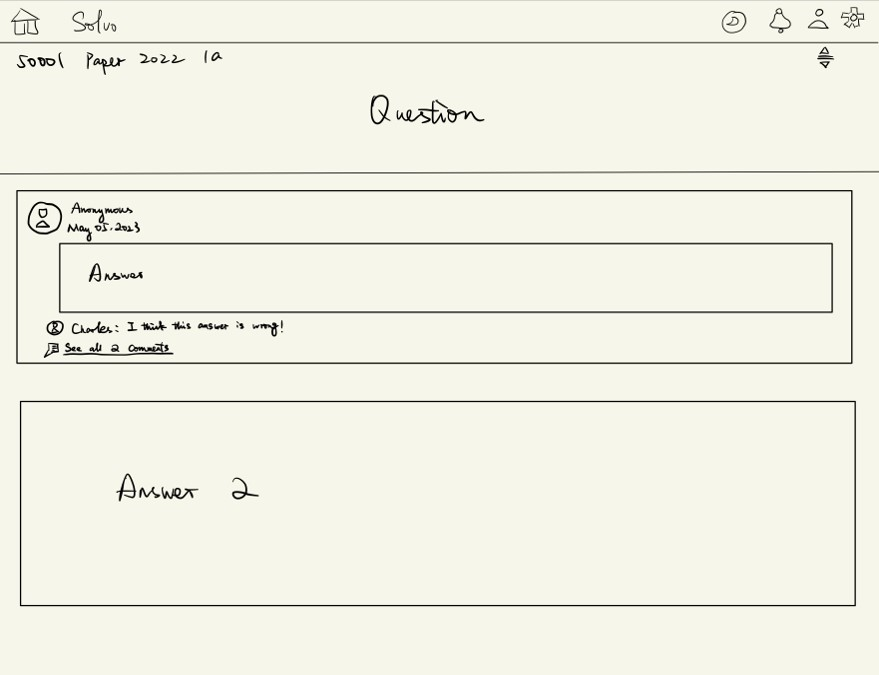
\includegraphics[width=\textwidth]{concept2}
                  \captionof*{figure}{Question page: concept}
    \end{minipage}\hspace{0.05\textwidth}
    \begin{minipage}{0.57\textwidth}
        \centering
        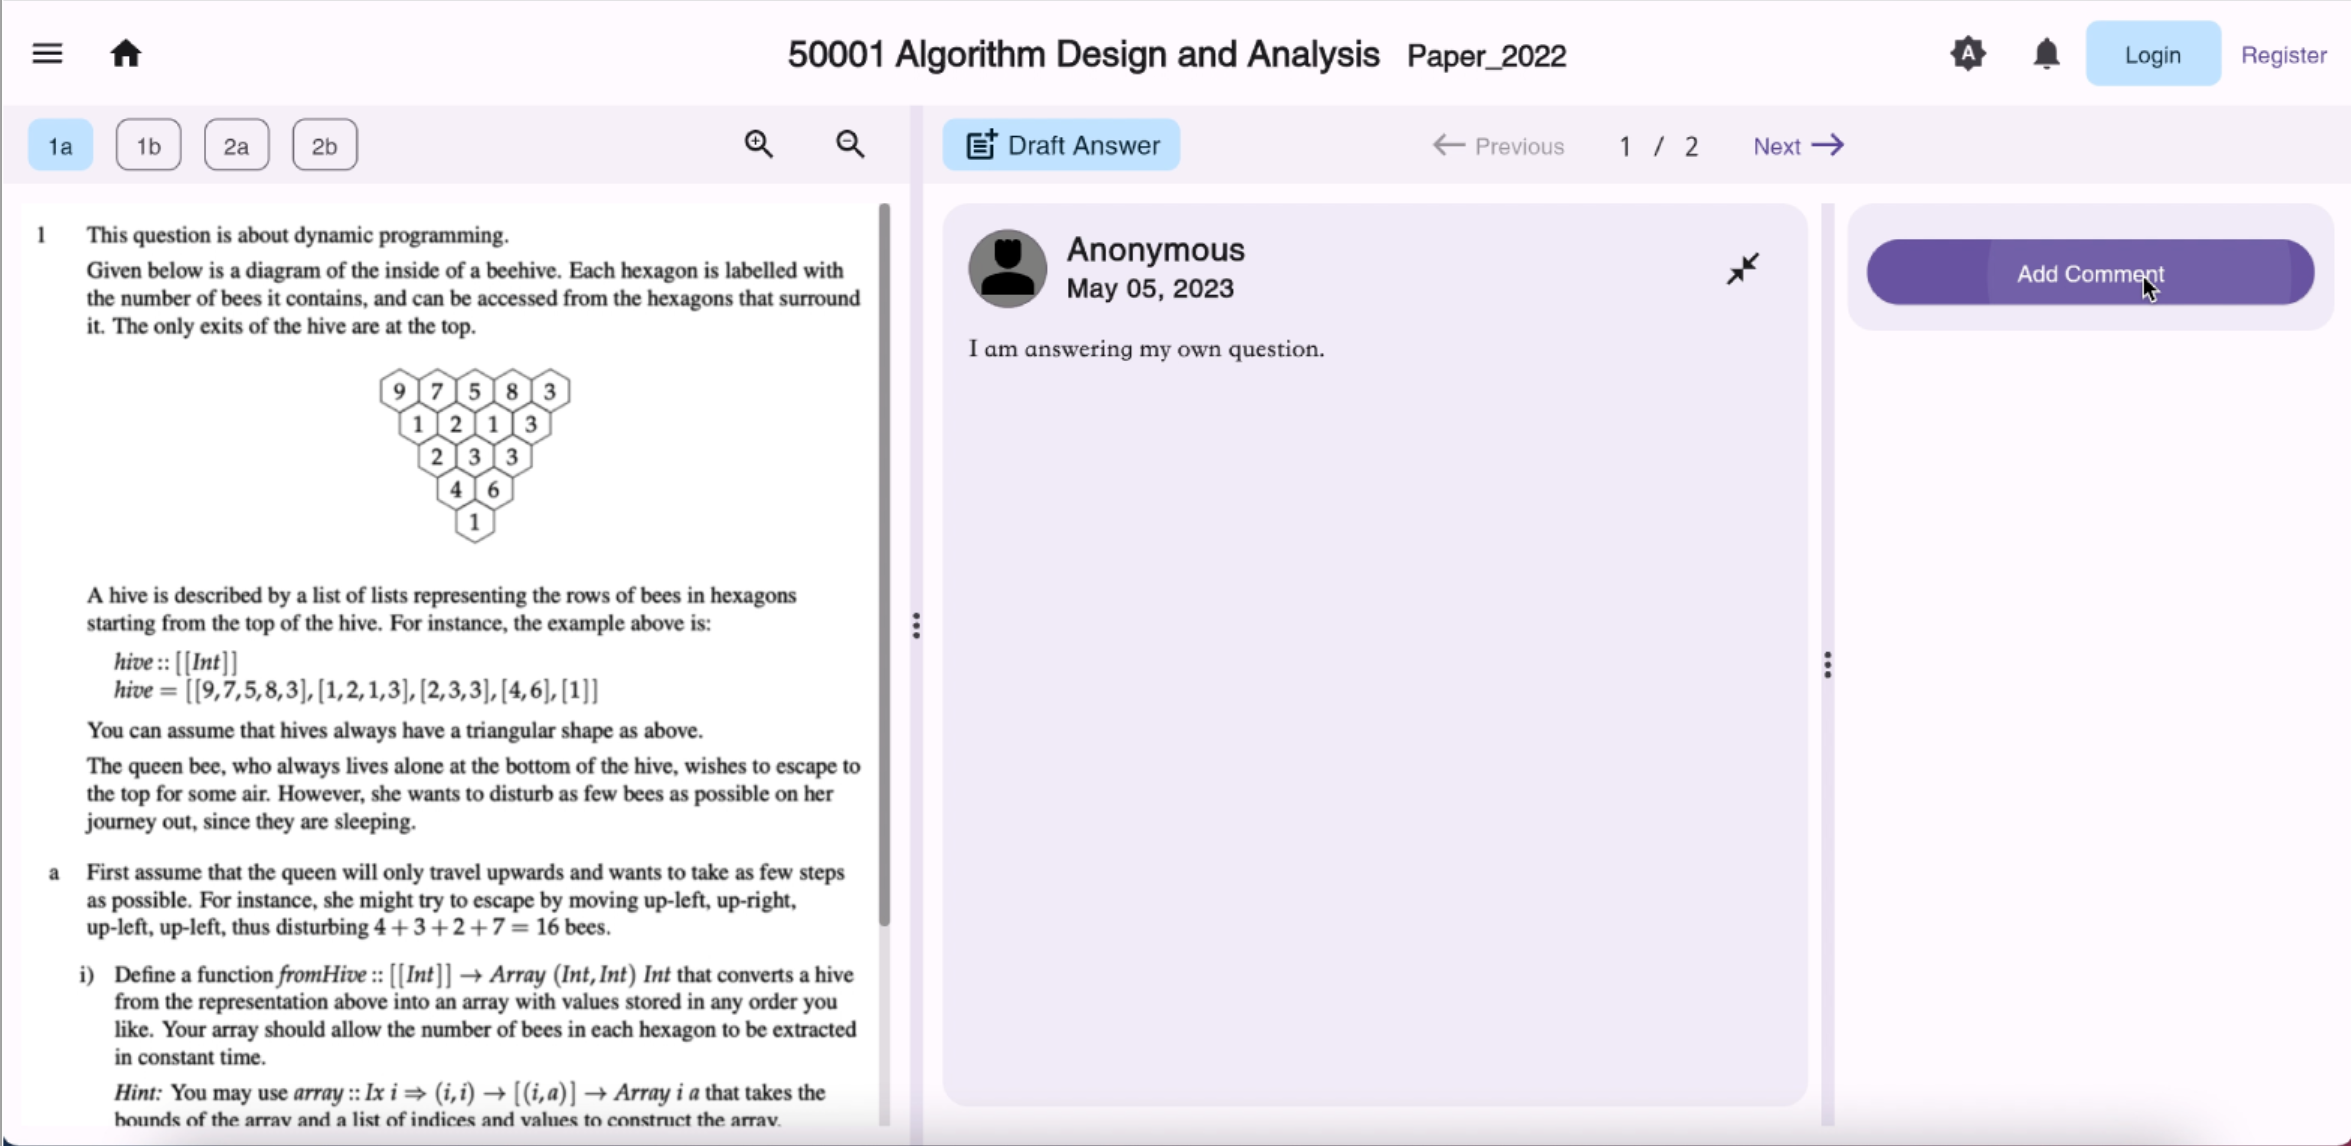
\includegraphics[width=\textwidth]{question-page1}
        \captionof*{figure}{Initial design}
    \end{minipage}

    \subsection*{Reaction System}
    \subsubsection*{Motivation}
    \noindent Users reflects that they are sometimes reluctant to post comments because:
    \begin{itemize}
        \item[-] ``Although sometimes I do feel like to leave some words, I'm just too lazy to think of the sentence and to type it out.''
        \item[-] ``Sometimes I want to express my agreement for someone's answer, but I think the comment area are for those thoughtful opinions,
        not for something like `you're right' `plus 1', so I would choose not to say anything.''
        \item[-] ``I am too shy to post my opinions on public platforms.
        It's better if you could have an anonymous system.''
    \end{itemize}

    To summarize, users tend to be lazy to type long comments, while short and less meaningful comments like ``you're right''
    seem to not quite fit into the comment area for some users.
    Some of them might be shy to post contents if we do not support anonymous posting.

    So our goal is to provide another way for users to give feedback to others, which is lighter and more convenient to use than comments,
    and is better to be anonymous.

    \subsubsection*{Design}
    A Reaction system is designed allowing viewers to quickly give feedback to answers by simply clicking on a button with emojis, instead of composing a text comment.
    The number of different emoji reactions received will be displayed at the bottom of the answer box.

    \begin{figure}[H]
        \centering
        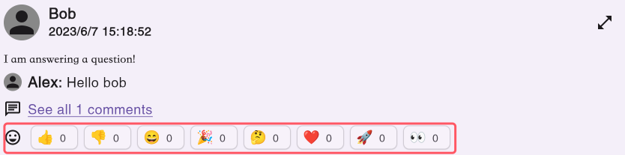
\includegraphics[width=0.8\textwidth]{reaction}
    \end{figure}

    \subsubsection*{Feedbacks and Reflection}
    \noindent We brought the design to users for validation, and most users agree that the feature makes them more motivated to give feedback to other's answers.
    \begin{itemize}
        \item[-] ``This is exactly what I want when I feel agreed with someone - without this I wouldn't want to post a comment.
        If I disagree with someone, though, I would probably click thumbs down and then post a comment explaining my ideas.''
        \item[-] ``As a person who posts answers, I would love to see feedbacks given in this way because these emojis are really straight forward and self-explanatory.
        It also provides diversity of the kind of feedbacks I can receive.''
    \end{itemize}

    The feature encourages users to give feedbacks to other's answers by providing a system that is easy to use and understand,
    and it could also benefit the ones who post answers because they can receive larger quantity of and more diverse feedbacks in this way.
    Therefore, it stimulates peer discussion on our platform, which is what we're targeting to achieve.

    \subsubsection*{Digital Touch-point Evolution}

    \begin{figure}[H]
        \centering
        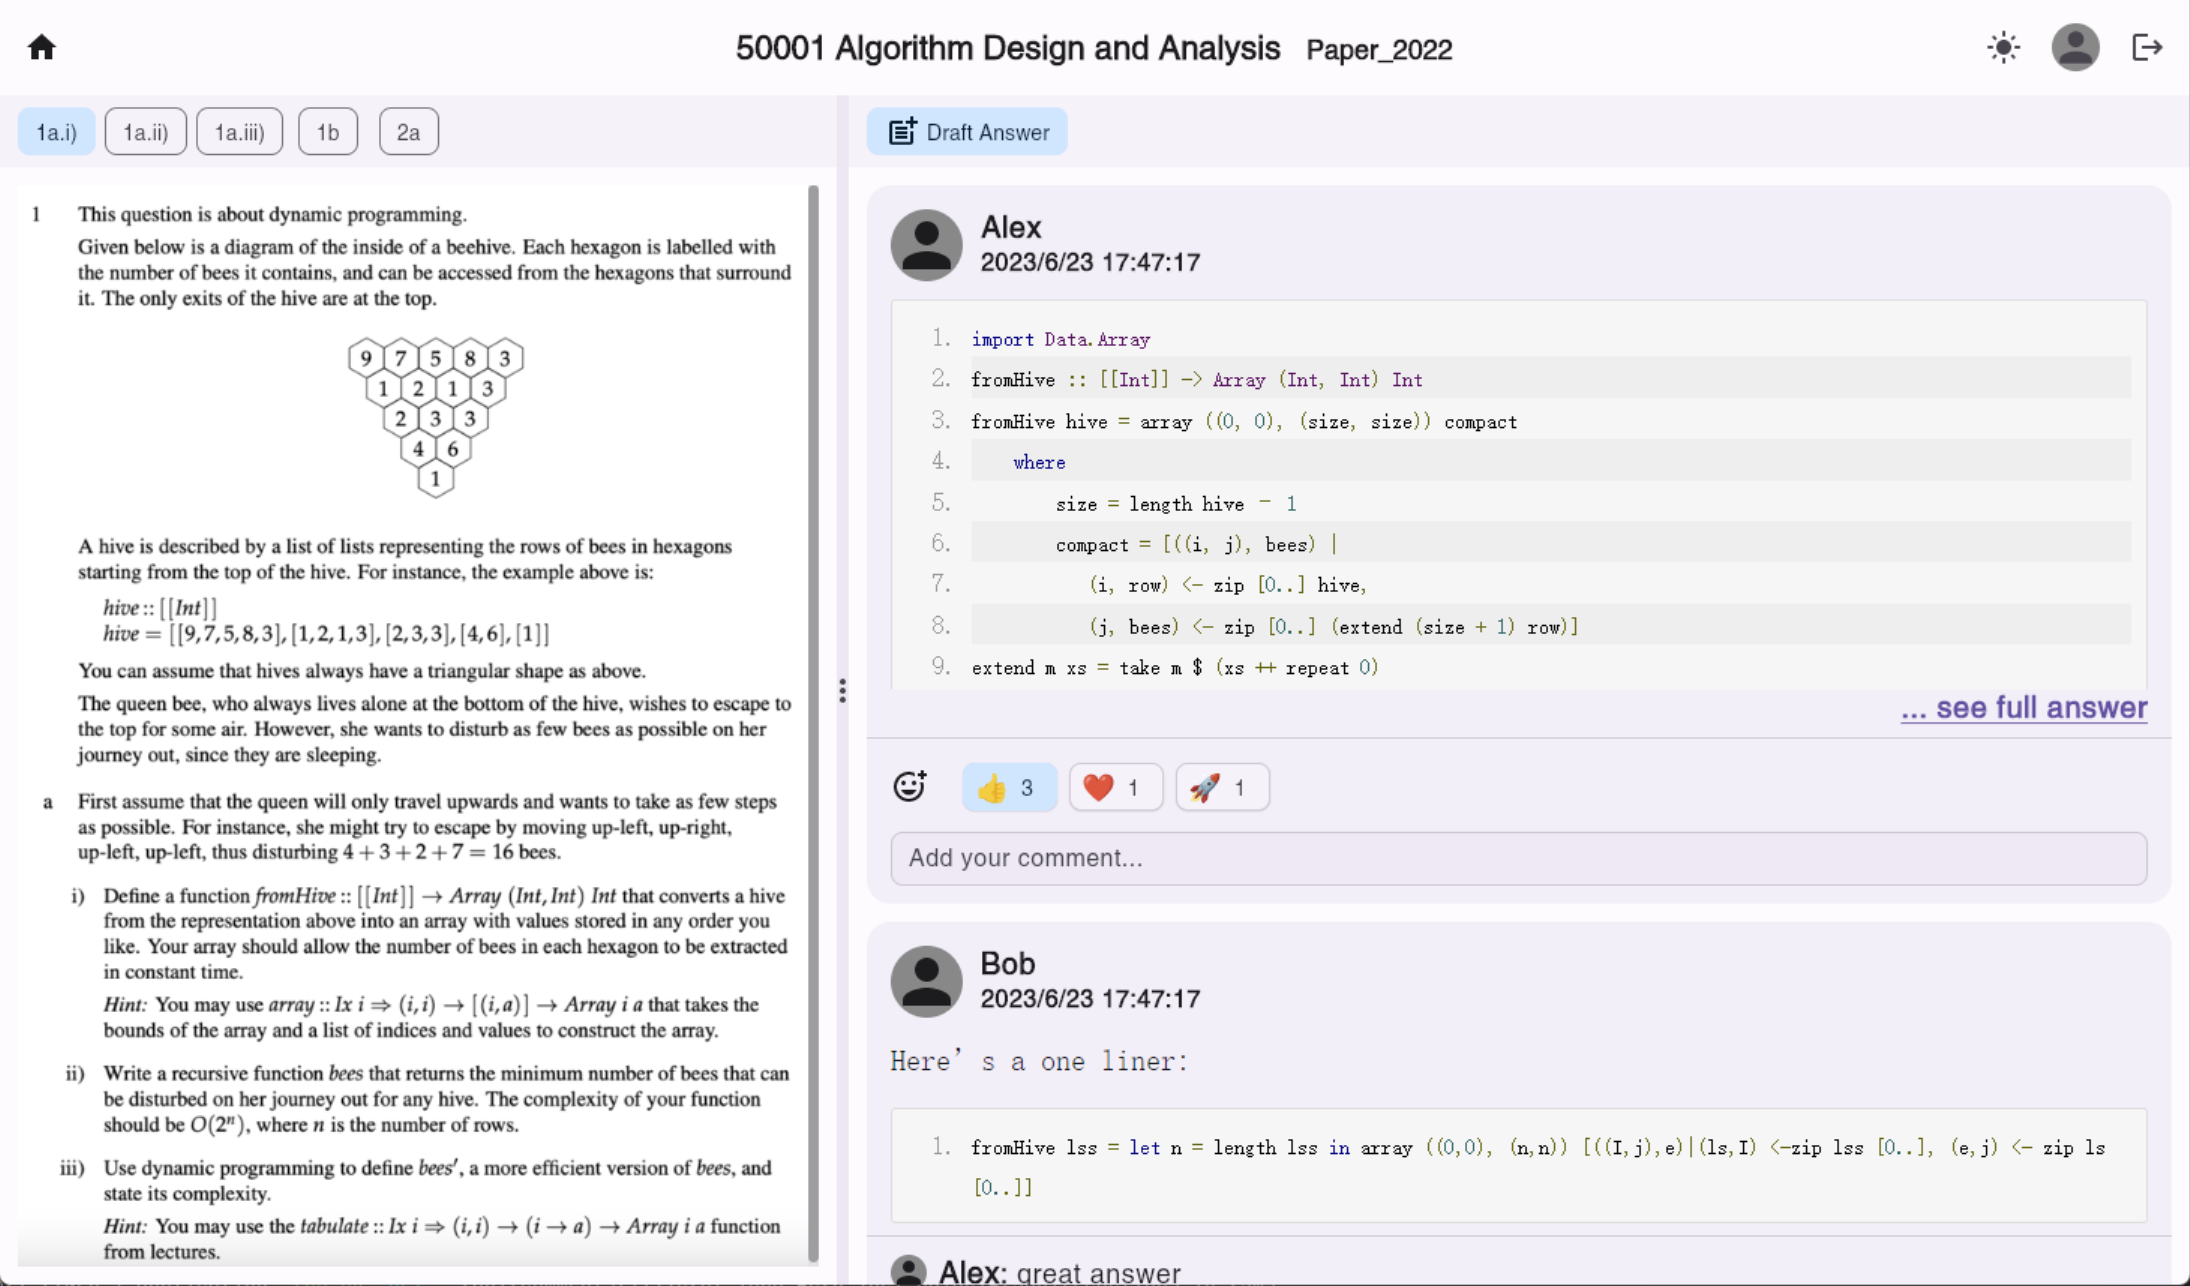
\includegraphics[width=0.8\textwidth]{question-page2}
        \\ Question page after adding reaction system
    \end{figure}

    \subsection*{Thoughts}

    \subsubsection*{Motivation}
    \noindent Users who seek answers on our platform suggests:
    \begin{itemize}
        \item[-] ``It's good if I can not only find answers to a question, but also others' thoughts and general ideas about a question.''
        \begin{itemize}
            \item[\textbullet] \textit{``Why is that?''}
            \item[-] ``Because viewing ideas from different people provides valuable insights, and gives me a much more comprehensive view of the question.''
        \end{itemize}
    \end{itemize}
    \noindent However, when we come to users who are willing to share answers, they indicate:
    \begin{itemize}
        \item[-] ``If I only have broad ideas or incomplete answers, I will definitely not post them,
        because I don't think these are qualified as a proper `answer', and may confuse others if I post them.''
        \item[-] ``Sometimes I don't feel like posting answers because I'm not confident about my answer.
        I'm worried that if my answer is wrong I could mislead other students.''
    \end{itemize}

    To summarize, users who seek answers would like to view ideas from different people besides detailed answers,
    but users who post answers will not post broad ideas or incomplete answers because they think those may confuse other students.
    Some are also worried about the correctness of their answers and are worried that they could mislead others.

    So our goal is to encourage users to share any of their thoughts and ideas, even if they do not have a full answer
    or are not sure about the correctness of it, while distinct such answers from complete answers to avoid confusion.

    \subsubsection*{Design}
    We add a line of text and a text button next to the "Draft Answer" button encouraging users to post their thoughts,
    and for answers that are posted in this way, a disclaimer is displayed in the top right corner of the answer box
    suggesting the content might not be complete or 100\% correct.

    \begin{figure}[H]
        \centering
        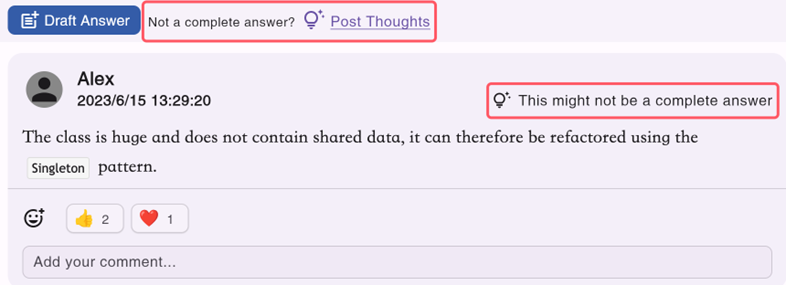
\includegraphics[width=0.8\textwidth]{thought1}
    \end{figure}

    \subsubsection*{Feedbacks and Iteration}
    \noindent We bring the initial design to users:

    \begin{itemize}
        \item \textit{``Suppose you are attempting this question, please try this.''}
        \begin{itemize}
            \item[-] (clicked reaction buttons and added a comment)
        \end{itemize}

        \item \textit{``Why didn't you use the 'Post Thoughts' button?''}
        \begin{itemize}
            \item[-] ``Which one? \ldots I didn't see that button.
            What's its functionality?''
        \end{itemize}

        \item
        \textit{``This is for you to share any general ideas, not limited to well-structured answers.
        Do you think you would be willing to use it if you understood this feature?''}
        \begin{itemize}
            \item[-] ``Yeah, if I only have some general ideas, I'll definitely not post an answer.
            But if I know that I can post `thoughts', I am glad to share them.''
        \end{itemize}
    \end{itemize}

    To summarize, most users did not notice the ``Post Thought'' button and does not understand its functionality.
    But after we explained to them the functionality of the button, they expressed that they are willing to use it to post thoughts
    if they could understand the feature.

    So our goal is to make the ``Post Thought' interaction more noticeable and easy to understand for users.

    In our next iteration, we changed the text button to a primary button and put it in parallel with the "Draft Answer" button.
    We also added a pop-up tip encouraging users to share their thoughts after they click a reaction button which shows up for 8 seconds.

    \begin{figure}[H]
        \centering
        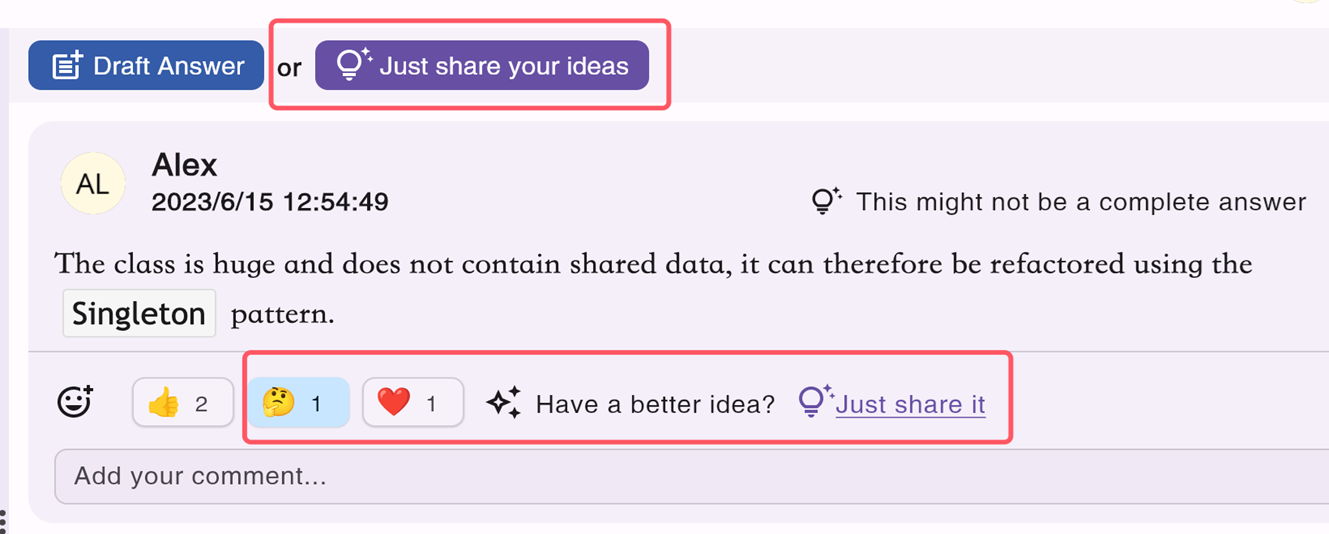
\includegraphics[width=0.8\textwidth]{thought2}
    \end{figure}

    \noindent Then we bring it back to users again.

    \begin{itemize}
        \item \textit{``Suppose you are attempting this question, please try this.''}
        \begin{itemize}
            \item[-] (Read through a wrong answer, clicked some reaction buttons and noticed the ``Have a better idea?'' pop-up. Then shared their own ideas)
        \end{itemize}
    \end{itemize}

    This time most users successfully noticed this feature and many of them are willing to share their own ideas.

    \subsubsection*{Reflection}

    The feature encourages users to share any of their ideas even if they are not sure about the details or correctness.
    This could provide more peer discussion on our platform, and therefore could benefit users that view answers
    by allowing them to view opinions from a wider range of people and gain a more comprehensive view of the question.

    \subsubsection*{Digital Touch-point Evolution}

    \begin{figure}[H]
        \centering
        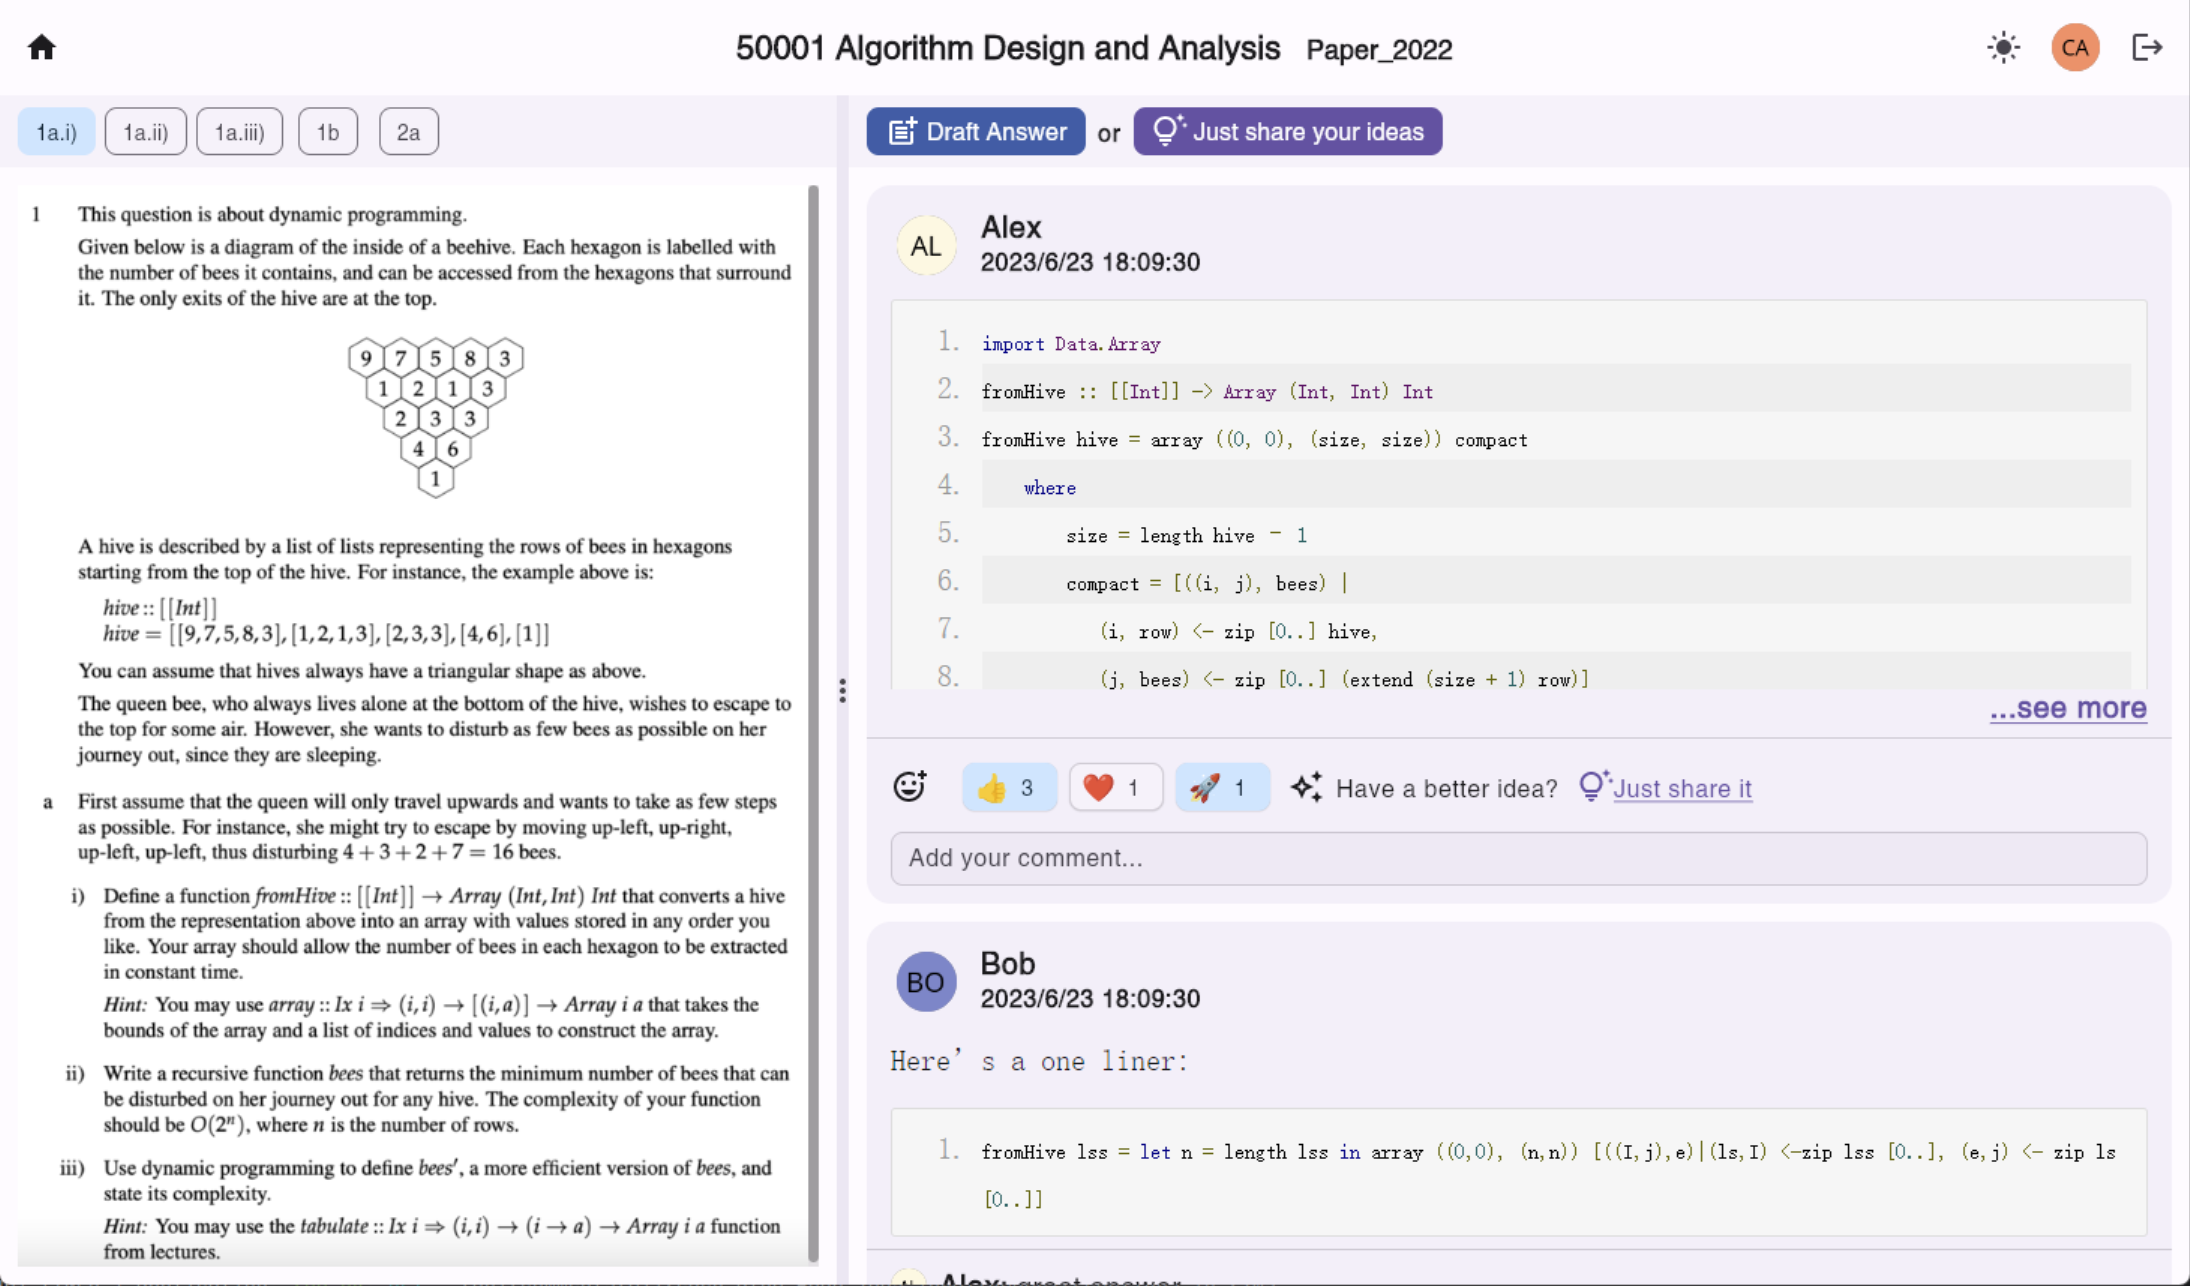
\includegraphics[width=0.8\textwidth]{question-page3}
        \\ Question page after adding thoughts
    \end{figure}

    \subsection*{Edit and Delete}

    \subsubsection*{Motivation}

    \noindent Users suggests that:
    \begin{itemize}
        \item[-] ``I may not want to post answers or share ideas if I can't modify them afterwards.
        I have to be very cautious about typos and stuff when writing posts, because I will not be able to change them later.''
        \item[-] ``Sometimes I don't feel like posting answers because I'm not confident about my answer.
        I'm worried that if my answer is wrong I could mislead other students.''
        \begin{itemize}
            \item[\textbullet] \textit{``Are there any improvements you could suggest to solve the problem you mentioned?''}
            \item[-] ``It's better to be able to edit or delete my content after I posted them, so that if I find that my previous
            answers are wrong, I could fix them so that they don't mislead other students.''
        \end{itemize}
    \end{itemize}

    To summarize, users are discouraged from posting contents if they can’t edit or delete them afterwards,
    because they have to be over-cautious about typos, or they are worried that if their answers are wrong that they can't fix it,
    other students may be misled by them.

    So our goal is to allow users to edit and delete contents they posted.

    \subsubsection*{Design}

    We add a three-dot button in the top right corner of the box of all current user's posts,
    which will expand and show the `Edit' and `Delete' button when clicked.

    \begin{figure}[H]
        \centering
        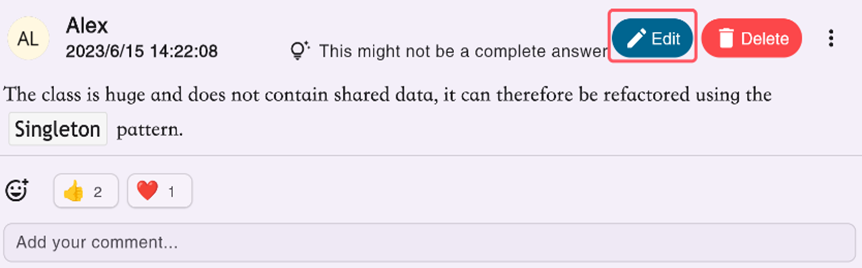
\includegraphics[width=0.8\textwidth]{edit}
    \end{figure}

    \subsubsection*{Feedbacks and Reflection}

    Users are generally satisfied with the functionality and interaction of this feature,
    and they do express stronger willingness to post answers and comments after we allowed them to edit and delete.

    \begin{itemize}
        \item[-] ``Yeah, being able to edit and delete my posts is indeed a crucial feature.
                   For me, I am much more willing to post things after you completed this feature.
                   \ldots I have no problems with the interaction of these buttons, too.''
    \end{itemize}

    As a reflection, allowing users to edit and delete what they posted could encourage them to make more posts and worry less
    about making mistakes and potentially misleading other students, and therefore could stimulate peer discussion on our platform.

    \subsubsection*{Digital Touch-point Evolution}

    \begin{figure}[H]
        \centering
        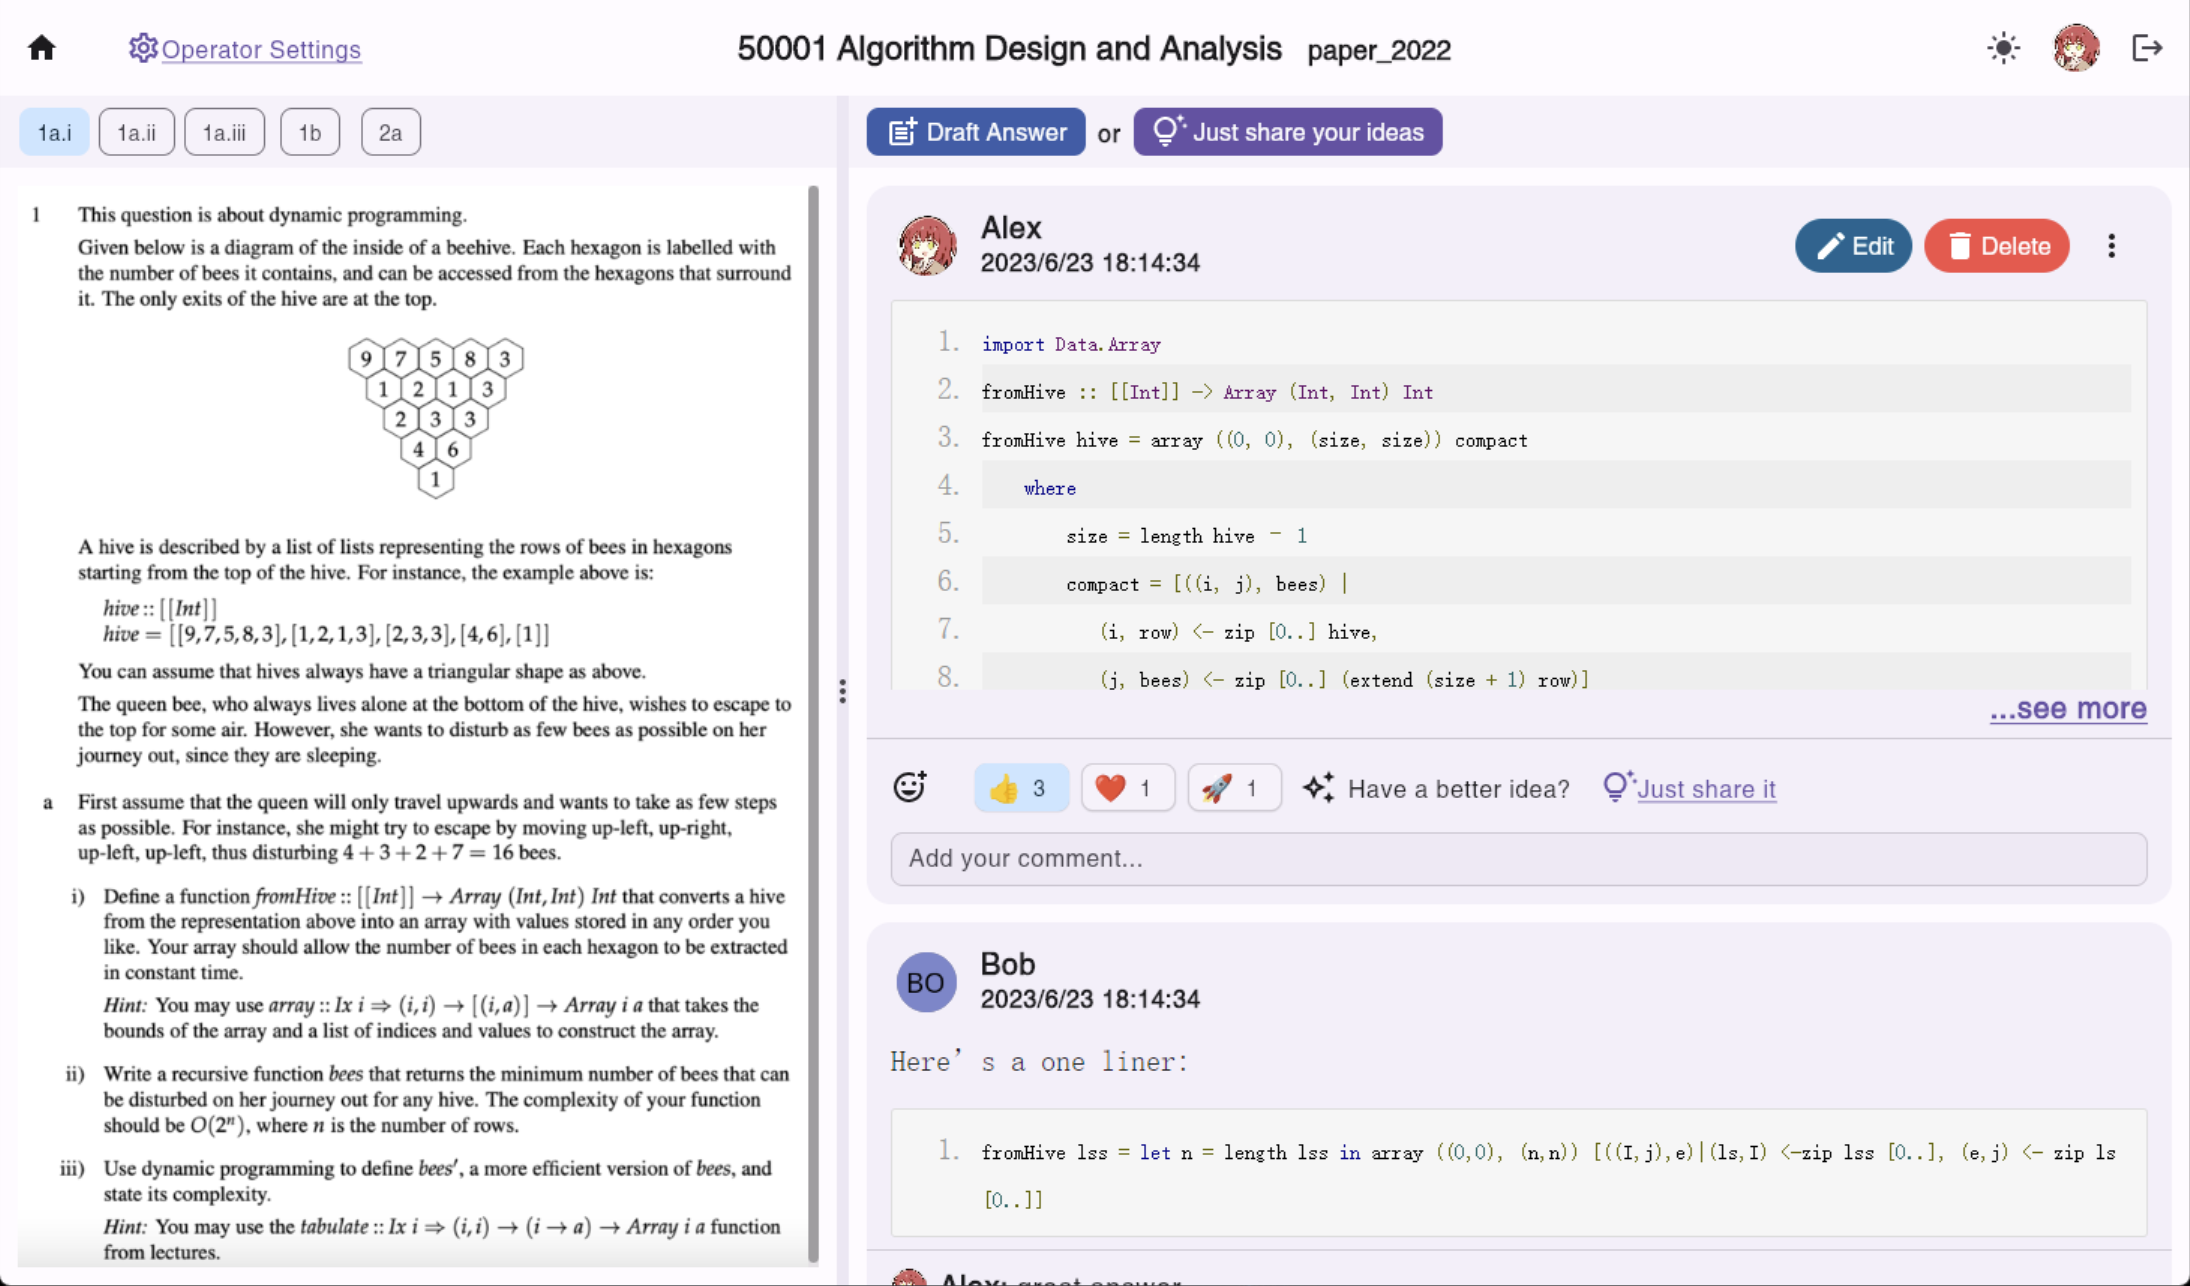
\includegraphics[width=0.8\textwidth]{question-page4}
        \\ Question page after adding edit and delete
    \end{figure}

    \section*{Impacts}

    \subsection*{Impact for Target Audience}

    \noindent Interviews were conducted to understand how Solvo can affect the stakeholders.

    We came back to students who used to discuss only with friends.
    The users responded with the following quotes:
    \begin{itemize}
        \item \textit{``Do you think you would be willing to use it if you understood this feature (the thoughts)?''}
        \begin{itemize}
            \item[-] ``Yeah, if I only have some general ideas, I will definitely not post an answer.
            But if I know that I can post \textbf{`Thoughts'}, I am \textbf{glad to share them}.''
        \end{itemize}

        \item
        \textit{``As a user, are you willing to give more feedback using the reaction system?''}
        \begin{itemize}
            \item[-] ``Yeah absolutely.''
            \item[-] ``I don’t want the comments to be filled up with meaningless comments like `+1'.
            With this reaction system, it can be much more clean.''
        \end{itemize}

        \item \textit{``Will you use the reactions?''}
        \begin{itemize}
            \item[-] ``Definitely.''
            \item[-] ``For me, I will write a comment only when I think the answer is incorrect.
            If I agree with the answer, I won't say `You are correct', which takes time.
            If there is no such quick reactions, I will just skip it.''
        \end{itemize}
    \end{itemize}

    Therefore, students \textbf{feel encouraged to share their ideas} because:
    \begin{itemize}
        \item it is clear that they can share `thoughts' rather than only complete answers;
        \item the comments are organized, so that adding a comment does not make it messy;
        \item they can use the reactions to quickly give feedback.
    \end{itemize}

    \begin{itemize}
        \item \textit{``Would you read the comments and reactions given by others? Why?''}
        \begin{itemize}
            \item[-] ``Yes, as they could be helpful.
            I can know I'm correct or wrong if people give me `thumb up' or `thumb dump'.
            Their comments may also give different views, so I may learn from them.''
        \end{itemize}

        \item \textit{``Try to work out this question, and verify your answer.''}
        \begin{itemize}
            \item[-] ``Okay.''
            \item[-] \ldots
        \end{itemize}
        \textit{``How do you like this experience?''}
        \begin{itemize}
            \item[-] ``Very nice, this is exactly what I want.
            The DoC Revision Folder is messy, and it's awful to navigate to multiple documents to read answers from different people.
            On Solvo it's much easier.''
        \end{itemize}
    \end{itemize}

    \noindent As it can be summarized from the quotes:

    On Solvo, students can also \textbf{share ideas with more people}, and \textbf{receive feedback} by the reactions and comments given by peers.
    They can know if they are appreciated by others, and \textbf{learn what they missed} in the past.

    \subsection*{Impact for Other Stakeholders}

    \noindent We interviewed five tutors from different institutions about their thoughts on Solvo.

    \begin{itemize}
        \item \textit{``Will you welcome your institution to introduce Solvo to students?''}
        \begin{itemize}
            \item[-] ``Of course.''
            \item[-] ``I love the peer discussion it (Solvo) provides.
            As a tutor, we always encourage students to discuss with each other and answer questions on the forum, even if it might be wrong.
            This allows them to learn from each other.''
        \end{itemize}
    \end{itemize}

    \noindent It is known from the interviews that tutors like the way Solvo promotes peer discussion, and are happy to welcome the introduction of Solvo.
    Although it is hard to verify, we may infer that tutors' workload can be reduced because of promoted peer discussion.

%    These connections can extend beyond the classroom and may lead to collaborations, study groups, or professional relationships that continue throughout their university experience and beyond.
\end{document}
